%%%%%%%%%%%%%%%%%%% author.tex %%%%%%%%%%%%%%%%%%%%%%%%%%%%%%%%%%%
%
% sample root file for your "contribution" to a contributed volume
%
% Use this file as a template for your own input.
%
%%%%%%%%%%%%%%%% Springer %%%%%%%%%%%%%%%%%%%%%%%%%%%%%%%%%%


% RECOMMENDED %%%%%%%%%%%%%%%%%%%%%%%%%%%%%%%%%%%%%%%%%%%%%%%%%%%
\documentclass[graybox]{svmult}

% choose options for [] as required from the list
% in the Reference Guide

\usepackage{mathptmx}       % selects Times Roman as basic font
\usepackage{helvet}         % selects Helvetica as sans-serif font
\usepackage{courier}        % selects Courier as typewriter font
\usepackage{type1cm}        % activate if the above 3 fonts are
                            % not available on your system
%
\usepackage{makeidx}         % allows index generation
\usepackage{graphicx}        % standard LaTeX graphics tool
                             % when including figure files
\usepackage{multicol}        % used for the two-column index
\usepackage[bottom]{footmisc}% places footnotes at page bottom
% see the list of further useful packages
% in the Reference Guide

\makeindex             % used for the subject index
                       % please use the style svind.ist with
                       % your makeindex program

%%%%%%%%%%%%%%%%%%%%%%%%%%%%%%%%%%%%%%%%%%%%%%%%%%%%%%%%%%%%%%%%%%%%%%%%%%%%%%%%%%%%%%%%%

\begin{document}

\title*{Contribution Title}
\author{Name of First Author and Name of Second Author}
\institute{Name of First Author \at Name, Address of Institute, \email{name@email.address}
\and Name of Second Author \at Name, Address of Institute \email{name@email.address}}
%
% Use the package "url.sty" to avoid
% problems with special characters
% used in your e-mail or web address
%
\maketitle

\abstract{We analyze G2 spot instance price}
\section{Introduction}\label{sec:1}
Explain opportunistic cloud computing resources with spot instance in EC2

Mention the difficulies of price change prediction
Ben-Yehuda et. al~\cite{spot-instance-pricing-analysis}

Describe uniqueness of GPU spot instance with DeepSpotCloud

Summarize the overall contents

\section{Time-Series Analysis for GPU Spot Instances}
List basic methods that are widely used in other wors

naive

mean

seasonal mean

ARIMA with different parameters

\section{Evaluation}
Compare all the methods of different types of algorithms to different instance types
\begin{figure}
\centering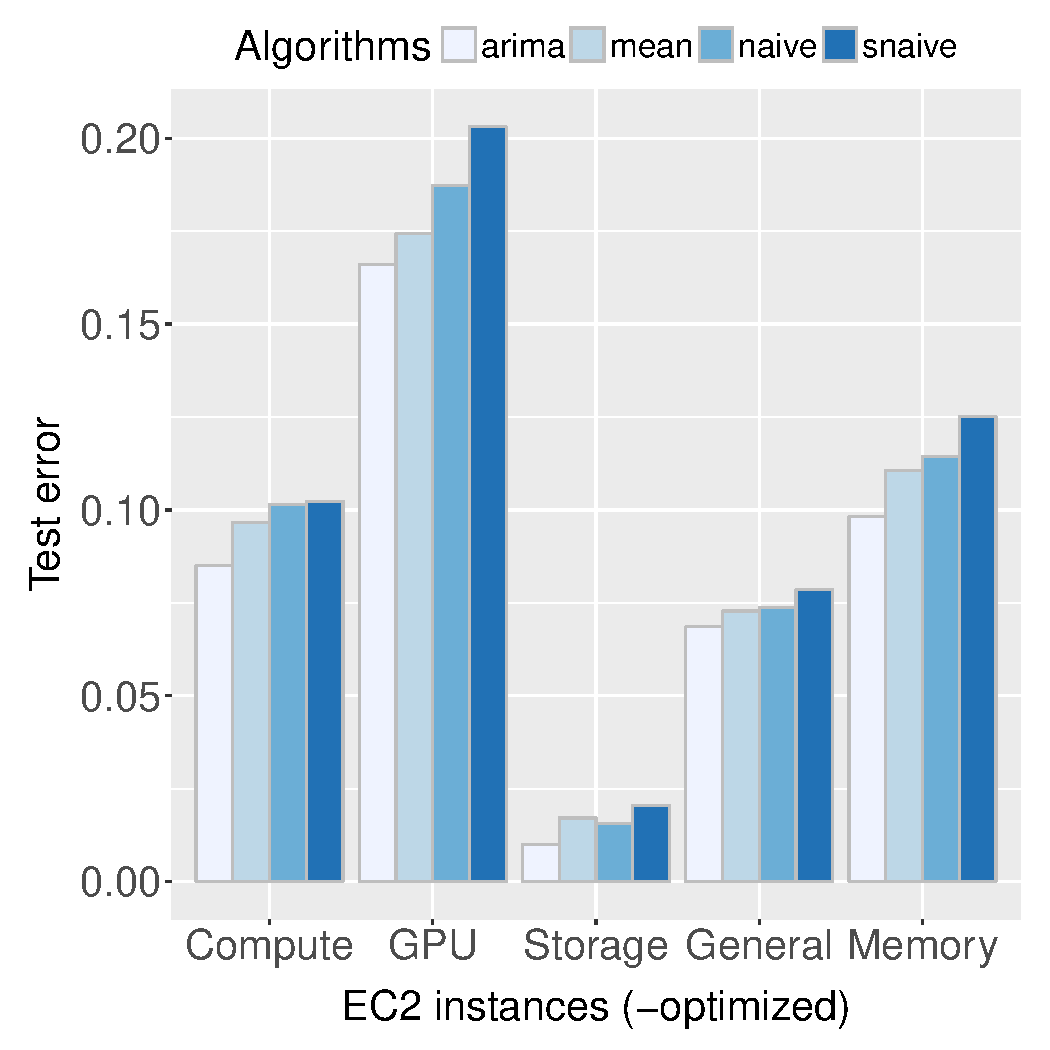
\includegraphics[width=0.7\textwidth]{figures/algorithm-compare-different-instance-type.pdf}\caption{Algorithms with different instance types\label{fig:algo-diff-inst}}
\end{figure}

\section{Conclusion}
Summarize

\begin{acknowledgement}
Thanks to ...
\end{acknowledgement}
\bibliographystyle{spmpsci}
\bibliography{g2-price-modeling}
\end{document}
